\chapter{Introduction}

This short tutorial consists of a set of small application targeted to
show the peculiarities of the main \ee\ API primitives.

The three applications described in this tutorial are the following:

\begin{description}
\item [Task API Example.] The example shows the main primitives about
  task management, including the options of preemptive and
  non-preemptive scheduling.

\item [Resource and Application Mode API Example.] The example shows
  the usage of the resource primitives and their interaction with the
  scheduling policies, as well as the usage of the Application Modes.

\item [Event and Alarm API Example.] The example shows how to use the
  primitives implementing event handling. It also shows the usage of
  \ee\ alarms, and the configuration of separate stacks for the
  application tasks.
\end{description}

The demos have been reported working with the following evaluation
board:

\begin{itemize}
\item Altera Stratix 1s40 evaluation Board
%% , \file{standard} example shipped with Altera Nios II.
\item Altera Stratix 2s60 RoHS evaluation Board
\end{itemize}

Other evaluation boards should work as well, because these examples
only use the following set of peripherals (which are normally included
in the examples provided by Altera):

\begin{itemize}
\item an Interval timer (the  System Clock) for periodic alarms;
\item a button;
\item an Avalon PIO with eight LEDs;
\item a JTAG UART.
\end{itemize}

Please report any problem, comment, and suggestion to the Evidence
technical support, by writing a mail to {\tt support@evidence.eu.com}.



\section{How to compile the demos}

This tutorial assumes the reader's familiarity with the Nios II IDE,
and the ability to create, compile and run an application using \ee.
However, in this section we provide a brief step-by-step guide to the setup and
usage of the main tools for running this tutorial.
%% The following paragraphs gives a quick overview of what needs to be done to run
%% an example. 
You can find more information on these topics in the \ee\ tutorial available in
the ERIKA Enterprise Reference Manual.



To compile and run the examples described in this document, follow the next steps:
\subsubsection{Installation of the development environment}
\begin{enumerate}
\item If you want to use the {\em Lauterbach Trace32 Debugger and Tracer}
\cite{Lauterbach} to flash and run the tutorial, copy the content
of the \file{files\\demo\\kernel\\orti} directory of the CDROM into
\file{C:\\t32\\demo\\kernel\\orti}.
\item Download the {\em Quartus II Web edition} environment from the {\em Altera} web site and
install the software on your computer.
\item Download the {\em Nios II IDE Web edition} environment from the {\em Altera} web site and
install the software on your computer.
\item Download the {\em Erika Enterprise and RT-Druid Demo Version for Altera Nios II}
from the {\em Evidence} website, and install the software on your computer.
\end{enumerate}


\subsubsection{Creation of the Jam images}
\begin{enumerate}
\item Start the {\em Quartus II} environment.
\item Click on {\em File} $\to$ {\em Open Project}.
\item Open the
\file{\C:\\altera\\80\\nios2eds\\examples\\...\\full_featured\\full_featured.qpf}\\
%% \file{\\full_featured.qpf} 
project.
\item Click on {\em Tools} $\to$ {Programmer}.
\item Check the {\em Prog/conf} checkbox.
\item Click on {\em File} $\to$ {\em Create/Update} $\to$ {\em Create JAM}.
\item Rename the file as \file{fpga.jam}\footnote{The file will be created in
\file{C:\\altera\\80\\nios2eds\\examples\\...\\full_featured}.}.
\item Save the project.

\item Click on {\em File} $\to$ {\em Open Project}.
\item Open the
\file{\C:\\altera\\80\\nios2eds\\examples\\...\\standard\\standard.qpf} project.
\item Click on {\em Tools} $\to$ {Programmer}.
\item Check the {\em Prog/conf} checkbox.
\item Click on {\em File} $\to$ {\em Create/Update} $\to$ {\em Create JAM}.
\item Rename the file as \file{fpga.jam}\footnote{The file will be created in
\file{C:\\altera\\80\\nios2eds\\examples\\...\\standard}.}.
\item Save the project.
\end{enumerate}


\subsubsection{Compiling the examples}
To run the examples, you need to create two
system libraries, one called \const{standard_syslib} (linked to the
\const{standard} example provided by Altera), the other called
\const{full_featured_syslib} (linked to the \const{full_featured}
example provided by Altera). 

Compile the examples in the following way:
\begin{enumerate}
\item Start the {\em Nios2 IDE} environment.
\item Click on {\em Windows} $\to$ {\em Preferences} $\to$ {\em RT-Druid} $\to$
{\em Oil} $\to$ {\em OS Configurator} and choose {\em Source distribution}.
\item Click on {\em New} $\to$ {\em Project} $\to$ {\em Altera Nios II} $\to$ {\em System Library}.
\item As project name, specify \file{standard_syslib}.
\item Build the project.

\item Click on {\em New} $\to$ {\em Project} $\to$ {\em Altera Nios II} $\to$ {\em System Library}.
\item As project name, specify \file{full_featured_syslib}.
\item Build the project.
\item Click on {\em New} $\to$ {\em Project} $\to$ {\em Evidence} $\to$ {\em RTDruid Oil and c/c++ project}.
\item Select one of the templates, as in Figure \ref{fig:newproject_nios2}

%
\begin{figure}
\begin{center}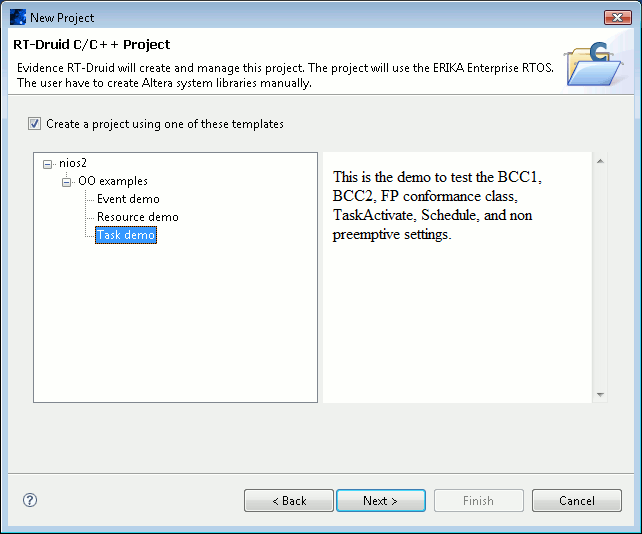
\includegraphics[%
  width=12cm, bb=0 0 642 534]{images/newproject_nios2.png}\end{center}
\caption{\label{fig:newproject_nios2} Creating a new project from a template.}
\end{figure}
%


\item As project name, specify \file{nios2_task}\footnote{For the \file{resource} and the \file{events} examples, just repeat these steps by creating a different project and importing the related files.}. 

\item Reference the two libraries already created (i.e. \file{standard_syslib}
and \file{full_featured_}\\ \file{syslib}).
\item Build the project\footnote{The ELF binary will be created in the
directory
\file{C:\\altera\\80\\nios2eds\\bin\\eclipse\\workspace\\}\\ \file{nios2_task\\Debug\\default_cpu}.}.
\item If you want to use the {\em Lauterbach Trace32 Debugger and Tracer}
\cite{Lauterbach} to flash and run the tutorial, run the \file{Debug.bat}
script and click on \file{go} once the T32 environment has finished
initialization.


%% \item Click on {\em New} $\to$ {\em Project} $\to$ {\em Evidence} $\to$ {\em RTDruid Oil and c/c++ project}.
%% \item As project name, specify \file{nios2_resource}.
%% \item Reference the two libraries already created (i.e. \file{standard_syslib} and \file{full_featured_syslib}).
%% \item Import the code from the \file{task} directory in the {\em EE API Tutorial for Nios 2}. 
%% Select {\em overwrite existing resources without warning}.
%% \item Build the project\footnote{The ELF binary will be created in the
%% directory
%% \file{C:\\altera\\kits\\nios2_60\\bin\\eclipse\\workspace\\}\\ \file{nios2_resource\\Debug\\default_cpu}.}.
%% \item If you want to use the {\em Lauterbach Trace32 Debugger and Tracer}
%% \cite{Lauterbach} to flash and run the tutorial, run the Debug.bat script and
%% click on go once the T32 environment has finished initialization.
%% 
%% \item Click on {\em New} $\to$ {\em Project} $\to$ {\em Evidence} $\to$ {\em RTDruid Oil and c/c++ project}.
%% \item As project name, specify \file{nios2_event}.
%% \item Reference the two libraries already created (i.e. \file{standard_syslib} and \file{full_featured_syslib}).
%% \item Import the code from the \file{task} directory in the {\em EE API Tutorial for Nios 2}. 
%% Select {\em overwrite existing resources without warning}.
%% \item Build the project \footnote{The ELF binary will be created in the
%% directory
%% \file{C:\\altera\\kits\\nios2_60\\bin\\eclipse\\workspace\\}\\ \file{nios2_event\\Debug\\default_cpu}.}.
%% \item If you want to use the {\em Lauterbach Trace32 Debugger and Tracer}
%% \cite{Lauterbach} to flash and run the tutorial, run the Debug.bat script and
%% click on go once the T32 environment has finished initialization.
\end{enumerate}

\begin{warning}
To run the examples as provided in this package without modifications,
you need to create the system libraries with the {\em same name and
location} as specified in the \const{SYSTEM_LIBRARY_NAME} and
\const{SYSTEM_LIBRARY_PATH} attributes in the OIL file provided with
each demo!
\end{warning}


%% \ee\ applications uses the Altera System Libraries as the base for
%% linker scripts, boot code and device drivers.  Open the Nios II IDE
%% from the rightmost tab in the SOPCBuilder tool and select {}``New''
%% from the File menu, and then ``Project...''. Choose {}``System
%% Library'' from the Altera Nios II tab of the New Project Dialog box.
%% 
%% 
%% 
%% Then, open the Nios II IDE from SOPCBuilder, and select ``New
%% Project...''  from the File menu. Choose ``RT-Druid Nios Project''
%% from the Evidence tab of the New Project Dialog box. A dialog box
%% appears.  Name the project with a meaningful name and press the Finish
%% button.
%% 
%% Select ``Import...'' from the File menu of the Nios II IDE. Select
%% ``File System'' from the dialog box. In the ``From directory''
%% textbox, type the name of the directory containing the example you
%% want to import. Choose the directory name in the tree view on the
%% left, selecting all the files on the right side. The ``Into Folder''
%% text box should point to the \rtd\ project just created. Finally,
%% select the checkbox ``Overwrite existing resources without warning''
%% and press Finish.



%% After that, right click on the project name, and select ``Build
%% Project''.  The demo application will be compiled, and an ELF binary
%% will be produced.

